% !TEX encoding = UTF-8 Unicode
\documentclass[10pt]{standalone}\usepackage{tikz}
\usepackage{fontspec}
\setmainfont{Arial}
\setsansfont{Arial}\begin{document}

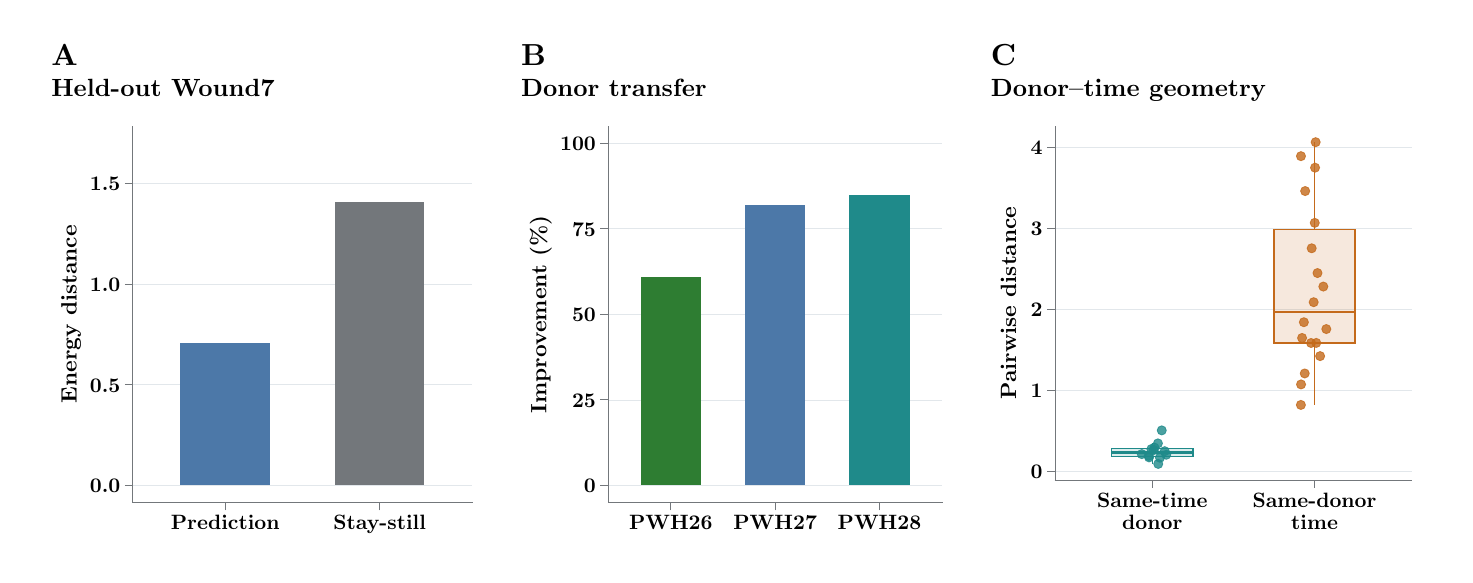
\begin{tikzpicture}[x=1pt,y=1pt]
\definecolor{fillColor}{RGB}{255,255,255}
\path[use as bounding box,fill=fillColor,fill opacity=0.00] (0,0) rectangle (512.15,190.63);
\begin{scope}
\path[clip] (  0.00,  0.00) rectangle (512.15,190.63);
\definecolor{drawColor}{RGB}{0,0,0}

\node[text=drawColor,anchor=base west,inner sep=0pt, outer sep=0pt, scale=  1.10] at (  8.54,177.07) {\bfseries A};

\node[text=drawColor,anchor=base west,inner sep=0pt, outer sep=0pt, scale=  0.90] at (  8.54,165.70) {\bfseries Held-out Wound7};
\end{scope}
\begin{scope}
\path[clip] (  8.54,  4.27) rectangle (164.08,160.19);
\definecolor{fillColor}{RGB}{255,255,255}

\path[fill=fillColor] (  8.54,  4.27) rectangle (164.08,160.19);
\end{scope}
\begin{scope}
\path[clip] ( 37.93, 19.07) rectangle (160.66,155.07);
\definecolor{fillColor}{RGB}{255,255,255}

\path[fill=fillColor] ( 37.93, 19.07) rectangle (160.66,155.07);
\definecolor{drawColor}{RGB}{226,231,235}

\path[draw=drawColor,line width= 0.2pt,line join=round] ( 37.93, 25.26) --
	(160.66, 25.26);

\path[draw=drawColor,line width= 0.2pt,line join=round] ( 37.93, 61.62) --
	(160.66, 61.62);

\path[draw=drawColor,line width= 0.2pt,line join=round] ( 37.93, 97.98) --
	(160.66, 97.98);

\path[draw=drawColor,line width= 0.2pt,line join=round] ( 37.93,134.34) --
	(160.66,134.34);
\definecolor{fillColor}{RGB}{76,120,168}

\path[fill=fillColor] ( 55.22, 25.26) rectangle ( 87.58, 76.55);
\definecolor{fillColor}{RGB}{115,119,123}

\path[fill=fillColor] (111.01, 25.26) rectangle (143.37,127.57);
\end{scope}
\begin{scope}
\path[clip] (  0.00,  0.00) rectangle (512.15,190.63);
\definecolor{drawColor}{RGB}{115,119,123}

\path[draw=drawColor,line width= 0.3pt,line join=round,line cap=rect] ( 37.93, 19.07) --
	( 37.93,155.07);
\end{scope}
\begin{scope}
\path[clip] (  0.00,  0.00) rectangle (512.15,190.63);
\definecolor{drawColor}{RGB}{0,0,0}

\node[text=drawColor,anchor=base east,inner sep=0pt, outer sep=0pt, scale=  0.75] at ( 33.49, 22.57) {\bfseries 0.0};

\node[text=drawColor,anchor=base east,inner sep=0pt, outer sep=0pt, scale=  0.75] at ( 33.49, 58.93) {\bfseries 0.5};

\node[text=drawColor,anchor=base east,inner sep=0pt, outer sep=0pt, scale=  0.75] at ( 33.49, 95.30) {\bfseries 1.0};

\node[text=drawColor,anchor=base east,inner sep=0pt, outer sep=0pt, scale=  0.75] at ( 33.49,131.66) {\bfseries 1.5};
\end{scope}
\begin{scope}
\path[clip] (  0.00,  0.00) rectangle (512.15,190.63);
\definecolor{drawColor}{RGB}{115,119,123}

\path[draw=drawColor,line width= 0.3pt,line join=round] ( 35.09, 25.26) --
	( 37.93, 25.26);

\path[draw=drawColor,line width= 0.3pt,line join=round] ( 35.09, 61.62) --
	( 37.93, 61.62);

\path[draw=drawColor,line width= 0.3pt,line join=round] ( 35.09, 97.98) --
	( 37.93, 97.98);

\path[draw=drawColor,line width= 0.3pt,line join=round] ( 35.09,134.34) --
	( 37.93,134.34);
\end{scope}
\begin{scope}
\path[clip] (  0.00,  0.00) rectangle (512.15,190.63);
\definecolor{drawColor}{RGB}{115,119,123}

\path[draw=drawColor,line width= 0.3pt,line join=round,line cap=rect] ( 37.93, 19.07) --
	(160.66, 19.07);
\end{scope}
\begin{scope}
\path[clip] (  0.00,  0.00) rectangle (512.15,190.63);
\definecolor{drawColor}{RGB}{115,119,123}

\path[draw=drawColor,line width= 0.3pt,line join=round] ( 71.40, 16.23) --
	( 71.40, 19.07);

\path[draw=drawColor,line width= 0.3pt,line join=round] (127.19, 16.23) --
	(127.19, 19.07);
\end{scope}
\begin{scope}
\path[clip] (  0.00,  0.00) rectangle (512.15,190.63);
\definecolor{drawColor}{RGB}{0,0,0}

\node[text=drawColor,anchor=base,inner sep=0pt, outer sep=0pt, scale=  0.75] at ( 71.40,  9.26) {\bfseries Prediction};

\node[text=drawColor,anchor=base,inner sep=0pt, outer sep=0pt, scale=  0.75] at (127.19,  9.26) {\bfseries Stay-still};
\end{scope}
\begin{scope}
\path[clip] (  0.00,  0.00) rectangle (512.15,190.63);
\definecolor{drawColor}{RGB}{0,0,0}

\node[text=drawColor,rotate= 90.00,anchor=base,inner sep=0pt, outer sep=0pt, scale=  0.80] at ( 17.68, 87.07) {\bfseries Energy distance};
\end{scope}
\begin{scope}
\path[clip] (  0.00,  0.00) rectangle (512.15,190.63);
\definecolor{drawColor}{RGB}{0,0,0}

\node[text=drawColor,anchor=base west,inner sep=0pt, outer sep=0pt, scale=  1.10] at (178.30,177.07) {\bfseries B};

\node[text=drawColor,anchor=base west,inner sep=0pt, outer sep=0pt, scale=  0.90] at (178.30,165.70) {\bfseries Donor transfer};
\end{scope}
\begin{scope}
\path[clip] (178.30,  4.27) rectangle (333.85,160.19);
\definecolor{fillColor}{RGB}{255,255,255}

\path[fill=fillColor] (178.30,  4.27) rectangle (333.85,160.19);
\end{scope}
\begin{scope}
\path[clip] (209.79, 19.07) rectangle (330.43,155.07);
\definecolor{fillColor}{RGB}{255,255,255}

\path[fill=fillColor] (209.79, 19.07) rectangle (330.43,155.07);
\definecolor{drawColor}{RGB}{226,231,235}

\path[draw=drawColor,line width= 0.2pt,line join=round] (209.79, 25.26) --
	(330.43, 25.26);

\path[draw=drawColor,line width= 0.2pt,line join=round] (209.79, 56.16) --
	(330.43, 56.16);

\path[draw=drawColor,line width= 0.2pt,line join=round] (209.79, 87.07) --
	(330.43, 87.07);

\path[draw=drawColor,line width= 0.2pt,line join=round] (209.79,117.98) --
	(330.43,117.98);

\path[draw=drawColor,line width= 0.2pt,line join=round] (209.79,148.89) --
	(330.43,148.89);
\definecolor{fillColor}{RGB}{46,125,50}

\path[fill=fillColor] (221.47, 25.26) rectangle (243.34,100.64);
\definecolor{fillColor}{RGB}{76,120,168}

\path[fill=fillColor] (259.18, 25.26) rectangle (281.04,126.45);
\definecolor{fillColor}{RGB}{31,138,138}

\path[fill=fillColor] (296.88, 25.26) rectangle (318.74,130.01);
\end{scope}
\begin{scope}
\path[clip] (  0.00,  0.00) rectangle (512.15,190.63);
\definecolor{drawColor}{RGB}{115,119,123}

\path[draw=drawColor,line width= 0.3pt,line join=round,line cap=rect] (209.79, 19.07) --
	(209.79,155.07);
\end{scope}
\begin{scope}
\path[clip] (  0.00,  0.00) rectangle (512.15,190.63);
\definecolor{drawColor}{RGB}{0,0,0}

\node[text=drawColor,anchor=base east,inner sep=0pt, outer sep=0pt, scale=  0.75] at (205.34, 22.57) {\bfseries 0};

\node[text=drawColor,anchor=base east,inner sep=0pt, outer sep=0pt, scale=  0.75] at (205.34, 53.48) {\bfseries 25};

\node[text=drawColor,anchor=base east,inner sep=0pt, outer sep=0pt, scale=  0.75] at (205.34, 84.39) {\bfseries 50};

\node[text=drawColor,anchor=base east,inner sep=0pt, outer sep=0pt, scale=  0.75] at (205.34,115.29) {\bfseries 75};

\node[text=drawColor,anchor=base east,inner sep=0pt, outer sep=0pt, scale=  0.75] at (205.34,146.20) {\bfseries 100};
\end{scope}
\begin{scope}
\path[clip] (  0.00,  0.00) rectangle (512.15,190.63);
\definecolor{drawColor}{RGB}{115,119,123}

\path[draw=drawColor,line width= 0.3pt,line join=round] (206.94, 25.26) --
	(209.79, 25.26);

\path[draw=drawColor,line width= 0.3pt,line join=round] (206.94, 56.16) --
	(209.79, 56.16);

\path[draw=drawColor,line width= 0.3pt,line join=round] (206.94, 87.07) --
	(209.79, 87.07);

\path[draw=drawColor,line width= 0.3pt,line join=round] (206.94,117.98) --
	(209.79,117.98);

\path[draw=drawColor,line width= 0.3pt,line join=round] (206.94,148.89) --
	(209.79,148.89);
\end{scope}
\begin{scope}
\path[clip] (  0.00,  0.00) rectangle (512.15,190.63);
\definecolor{drawColor}{RGB}{115,119,123}

\path[draw=drawColor,line width= 0.3pt,line join=round,line cap=rect] (209.79, 19.07) --
	(330.43, 19.07);
\end{scope}
\begin{scope}
\path[clip] (  0.00,  0.00) rectangle (512.15,190.63);
\definecolor{drawColor}{RGB}{115,119,123}

\path[draw=drawColor,line width= 0.3pt,line join=round] (232.41, 16.23) --
	(232.41, 19.07);

\path[draw=drawColor,line width= 0.3pt,line join=round] (270.11, 16.23) --
	(270.11, 19.07);

\path[draw=drawColor,line width= 0.3pt,line join=round] (307.81, 16.23) --
	(307.81, 19.07);
\end{scope}
\begin{scope}
\path[clip] (  0.00,  0.00) rectangle (512.15,190.63);
\definecolor{drawColor}{RGB}{0,0,0}

\node[text=drawColor,anchor=base,inner sep=0pt, outer sep=0pt, scale=  0.75] at (232.41,  9.26) {\bfseries PWH26};

\node[text=drawColor,anchor=base,inner sep=0pt, outer sep=0pt, scale=  0.75] at (270.11,  9.26) {\bfseries PWH27};

\node[text=drawColor,anchor=base,inner sep=0pt, outer sep=0pt, scale=  0.75] at (307.81,  9.26) {\bfseries PWH28};
\end{scope}
\begin{scope}
\path[clip] (  0.00,  0.00) rectangle (512.15,190.63);
\definecolor{drawColor}{RGB}{0,0,0}

\node[text=drawColor,rotate= 90.00,anchor=base,inner sep=0pt, outer sep=0pt, scale=  0.80] at (187.44, 87.07) {\bfseries Improvement ({\%})};
\end{scope}
\begin{scope}
\path[clip] (  0.00,  0.00) rectangle (512.15,190.63);
\definecolor{drawColor}{RGB}{0,0,0}

\node[text=drawColor,anchor=base west,inner sep=0pt, outer sep=0pt, scale=  1.10] at (348.07,177.07) {\bfseries C};

\node[text=drawColor,anchor=base west,inner sep=0pt, outer sep=0pt, scale=  0.90] at (348.07,165.70) {\bfseries Donor–time geometry};
\end{scope}
\begin{scope}
\path[clip] (348.07,  4.27) rectangle (503.61,160.19);
\definecolor{fillColor}{RGB}{255,255,255}

\path[fill=fillColor] (348.07,  4.27) rectangle (503.61,160.19);
\end{scope}
\begin{scope}
\path[clip] (371.21, 27.17) rectangle (500.20,155.07);
\definecolor{fillColor}{RGB}{255,255,255}

\path[fill=fillColor] (371.21, 27.17) rectangle (500.20,155.07);
\definecolor{drawColor}{RGB}{226,231,235}

\path[draw=drawColor,line width= 0.2pt,line join=round] (371.21, 30.26) --
	(500.20, 30.26);

\path[draw=drawColor,line width= 0.2pt,line join=round] (371.21, 59.53) --
	(500.20, 59.53);

\path[draw=drawColor,line width= 0.2pt,line join=round] (371.21, 88.80) --
	(500.20, 88.80);

\path[draw=drawColor,line width= 0.2pt,line join=round] (371.21,118.07) --
	(500.20,118.07);

\path[draw=drawColor,line width= 0.2pt,line join=round] (371.21,147.34) --
	(500.20,147.34);
\definecolor{drawColor}{RGB}{31,138,138}

\path[draw=drawColor,line width= 0.5pt,line join=round] (406.39, 38.49) -- (406.39, 40.41);

\path[draw=drawColor,line width= 0.5pt,line join=round] (406.39, 35.76) -- (406.39, 32.99);
\definecolor{fillColor}{RGB}{31,138,138}

\path[draw=drawColor,line width= 0.5pt,fill=fillColor,fill opacity=0.15] (391.73, 38.49) --
	(391.73, 35.76) --
	(421.05, 35.76) --
	(421.05, 38.49) --
	(391.73, 38.49) --
	cycle;

\path[draw=drawColor,line width= 0.9pt] (391.73, 37.07) -- (421.05, 37.07);
\definecolor{drawColor}{RGB}{196,106,27}

\path[draw=drawColor,line width= 0.5pt,line join=round] (465.02,117.80) -- (465.02,149.25);

\path[draw=drawColor,line width= 0.5pt,line join=round] (465.02, 76.70) -- (465.02, 54.31);
\definecolor{fillColor}{RGB}{196,106,27}

\path[draw=drawColor,line width= 0.5pt,fill=fillColor,fill opacity=0.15] (450.36,117.80) --
	(450.36, 76.70) --
	(479.68, 76.70) --
	(479.68,117.80) --
	(450.36,117.80) --
	cycle;

\path[draw=drawColor,line width= 0.9pt] (450.36, 87.82) -- (479.68, 87.82);
\definecolor{drawColor}{RGB}{31,138,138}
\definecolor{fillColor}{RGB}{31,138,138}

\path[draw=drawColor,draw opacity=0.80,line width= 0.3pt,line join=round,line cap=round,fill=fillColor,fill opacity=0.80] (411.42, 36.30) circle (  1.65);

\path[draw=drawColor,draw opacity=0.80,line width= 0.3pt,line join=round,line cap=round,fill=fillColor,fill opacity=0.80] (405.06, 35.90) circle (  1.65);

\path[draw=drawColor,draw opacity=0.80,line width= 0.3pt,line join=round,line cap=round,fill=fillColor,fill opacity=0.80] (409.15, 35.22) circle (  1.65);

\path[draw=drawColor,draw opacity=0.80,line width= 0.3pt,line join=round,line cap=round,fill=fillColor,fill opacity=0.80] (409.79, 45.11) circle (  1.65);

\path[draw=drawColor,draw opacity=0.80,line width= 0.3pt,line join=round,line cap=round,fill=fillColor,fill opacity=0.80] (407.17, 38.89) circle (  1.65);

\path[draw=drawColor,draw opacity=0.80,line width= 0.3pt,line join=round,line cap=round,fill=fillColor,fill opacity=0.80] (408.41, 40.41) circle (  1.65);

\path[draw=drawColor,draw opacity=0.80,line width= 0.3pt,line join=round,line cap=round,fill=fillColor,fill opacity=0.80] (405.22, 35.35) circle (  1.65);

\path[draw=drawColor,draw opacity=0.80,line width= 0.3pt,line join=round,line cap=round,fill=fillColor,fill opacity=0.80] (406.06, 38.36) circle (  1.65);

\path[draw=drawColor,draw opacity=0.80,line width= 0.3pt,line join=round,line cap=round,fill=fillColor,fill opacity=0.80] (406.85, 37.98) circle (  1.65);

\path[draw=drawColor,draw opacity=0.80,line width= 0.3pt,line join=round,line cap=round,fill=fillColor,fill opacity=0.80] (410.87, 37.59) circle (  1.65);

\path[draw=drawColor,draw opacity=0.80,line width= 0.3pt,line join=round,line cap=round,fill=fillColor,fill opacity=0.80] (402.58, 36.54) circle (  1.65);

\path[draw=drawColor,draw opacity=0.80,line width= 0.3pt,line join=round,line cap=round,fill=fillColor,fill opacity=0.80] (408.52, 32.99) circle (  1.65);
\definecolor{drawColor}{RGB}{196,106,27}
\definecolor{fillColor}{RGB}{196,106,27}

\path[draw=drawColor,draw opacity=0.80,line width= 0.3pt,line join=round,line cap=round,fill=fillColor,fill opacity=0.80] (461.46, 65.68) circle (  1.65);

\path[draw=drawColor,draw opacity=0.80,line width= 0.3pt,line join=round,line cap=round,fill=fillColor,fill opacity=0.80] (466.07,101.96) circle (  1.65);

\path[draw=drawColor,draw opacity=0.80,line width= 0.3pt,line join=round,line cap=round,fill=fillColor,fill opacity=0.80] (465.08,120.10) circle (  1.65);

\path[draw=drawColor,draw opacity=0.80,line width= 0.3pt,line join=round,line cap=round,fill=fillColor,fill opacity=0.80] (469.26, 81.72) circle (  1.65);

\path[draw=drawColor,draw opacity=0.80,line width= 0.3pt,line join=round,line cap=round,fill=fillColor,fill opacity=0.80] (463.97,110.91) circle (  1.65);

\path[draw=drawColor,draw opacity=0.80,line width= 0.3pt,line join=round,line cap=round,fill=fillColor,fill opacity=0.80] (460.07, 54.31) circle (  1.65);

\path[draw=drawColor,draw opacity=0.80,line width= 0.3pt,line join=round,line cap=round,fill=fillColor,fill opacity=0.80] (460.50, 78.51) circle (  1.65);

\path[draw=drawColor,draw opacity=0.80,line width= 0.3pt,line join=round,line cap=round,fill=fillColor,fill opacity=0.80] (464.69, 91.43) circle (  1.65);

\path[draw=drawColor,draw opacity=0.80,line width= 0.3pt,line join=round,line cap=round,fill=fillColor,fill opacity=0.80] (461.62,131.59) circle (  1.65);

\path[draw=drawColor,draw opacity=0.80,line width= 0.3pt,line join=round,line cap=round,fill=fillColor,fill opacity=0.80] (465.62, 76.72) circle (  1.65);

\path[draw=drawColor,draw opacity=0.80,line width= 0.3pt,line join=round,line cap=round,fill=fillColor,fill opacity=0.80] (465.19,140.04) circle (  1.65);

\path[draw=drawColor,draw opacity=0.80,line width= 0.3pt,line join=round,line cap=round,fill=fillColor,fill opacity=0.80] (461.15, 84.20) circle (  1.65);

\path[draw=drawColor,draw opacity=0.80,line width= 0.3pt,line join=round,line cap=round,fill=fillColor,fill opacity=0.80] (467.02, 71.95) circle (  1.65);

\path[draw=drawColor,draw opacity=0.80,line width= 0.3pt,line join=round,line cap=round,fill=fillColor,fill opacity=0.80] (463.75, 76.69) circle (  1.65);

\path[draw=drawColor,draw opacity=0.80,line width= 0.3pt,line join=round,line cap=round,fill=fillColor,fill opacity=0.80] (460.10,144.20) circle (  1.65);

\path[draw=drawColor,draw opacity=0.80,line width= 0.3pt,line join=round,line cap=round,fill=fillColor,fill opacity=0.80] (460.13, 61.72) circle (  1.65);

\path[draw=drawColor,draw opacity=0.80,line width= 0.3pt,line join=round,line cap=round,fill=fillColor,fill opacity=0.80] (465.41,149.25) circle (  1.65);

\path[draw=drawColor,draw opacity=0.80,line width= 0.3pt,line join=round,line cap=round,fill=fillColor,fill opacity=0.80] (468.18, 97.08) circle (  1.65);
\end{scope}
\begin{scope}
\path[clip] (  0.00,  0.00) rectangle (512.15,190.63);
\definecolor{drawColor}{RGB}{115,119,123}

\path[draw=drawColor,line width= 0.3pt,line join=round,line cap=rect] (371.21, 27.17) --
	(371.21,155.07);
\end{scope}
\begin{scope}
\path[clip] (  0.00,  0.00) rectangle (512.15,190.63);
\definecolor{drawColor}{RGB}{0,0,0}

\node[text=drawColor,anchor=base east,inner sep=0pt, outer sep=0pt, scale=  0.75] at (366.77, 27.57) {\bfseries 0};

\node[text=drawColor,anchor=base east,inner sep=0pt, outer sep=0pt, scale=  0.75] at (366.77, 56.84) {\bfseries 1};

\node[text=drawColor,anchor=base east,inner sep=0pt, outer sep=0pt, scale=  0.75] at (366.77, 86.11) {\bfseries 2};

\node[text=drawColor,anchor=base east,inner sep=0pt, outer sep=0pt, scale=  0.75] at (366.77,115.38) {\bfseries 3};

\node[text=drawColor,anchor=base east,inner sep=0pt, outer sep=0pt, scale=  0.75] at (366.77,144.65) {\bfseries 4};
\end{scope}
\begin{scope}
\path[clip] (  0.00,  0.00) rectangle (512.15,190.63);
\definecolor{drawColor}{RGB}{115,119,123}

\path[draw=drawColor,line width= 0.3pt,line join=round] (368.37, 30.26) --
	(371.21, 30.26);

\path[draw=drawColor,line width= 0.3pt,line join=round] (368.37, 59.53) --
	(371.21, 59.53);

\path[draw=drawColor,line width= 0.3pt,line join=round] (368.37, 88.80) --
	(371.21, 88.80);

\path[draw=drawColor,line width= 0.3pt,line join=round] (368.37,118.07) --
	(371.21,118.07);

\path[draw=drawColor,line width= 0.3pt,line join=round] (368.37,147.34) --
	(371.21,147.34);
\end{scope}
\begin{scope}
\path[clip] (  0.00,  0.00) rectangle (512.15,190.63);
\definecolor{drawColor}{RGB}{115,119,123}

\path[draw=drawColor,line width= 0.3pt,line join=round,line cap=rect] (371.21, 27.17) --
	(500.20, 27.17);
\end{scope}
\begin{scope}
\path[clip] (  0.00,  0.00) rectangle (512.15,190.63);
\definecolor{drawColor}{RGB}{115,119,123}

\path[draw=drawColor,line width= 0.3pt,line join=round] (406.39, 24.33) --
	(406.39, 27.17);

\path[draw=drawColor,line width= 0.3pt,line join=round] (465.02, 24.33) --
	(465.02, 27.17);
\end{scope}
\begin{scope}
\path[clip] (  0.00,  0.00) rectangle (512.15,190.63);
\definecolor{drawColor}{RGB}{0,0,0}

\node[text=drawColor,anchor=base,inner sep=0pt, outer sep=0pt, scale=  0.75] at (406.39, 17.36) {\bfseries Same-time};

\node[text=drawColor,anchor=base,inner sep=0pt, outer sep=0pt, scale=  0.75] at (406.39,  9.26) {\bfseries donor};

\node[text=drawColor,anchor=base,inner sep=0pt, outer sep=0pt, scale=  0.75] at (465.02, 17.36) {\bfseries Same-donor};

\node[text=drawColor,anchor=base,inner sep=0pt, outer sep=0pt, scale=  0.75] at (465.02,  9.26) {\bfseries time};
\end{scope}
\begin{scope}
\path[clip] (  0.00,  0.00) rectangle (512.15,190.63);
\definecolor{drawColor}{RGB}{0,0,0}

\node[text=drawColor,rotate= 90.00,anchor=base,inner sep=0pt, outer sep=0pt, scale=  0.80] at (357.21, 91.12) {\bfseries Pairwise distance};
\end{scope}
\end{tikzpicture}

\end{document}
